
\blinddocument

\chapter{Mathematische Formeln}\label{cha:mathematischeFormeln}

\blindmathpaper

\chapter{Formatierungen}\label{cha:formatierungen}

\blindtext

\section{Text}\label{sec:text}

Zum guten Style gehört:
\begin{itemize}
	\item Versuche alle Warnungen beim erstellen zu beheben
	\item Zu einem Chapter, Section, Grafik, Tabelle, ... gehört immer ein \textit{caption} und \textit{label}
\end{itemize}

Umlaute können einfach benutzt werden z.B. äÖü. Hingegen mu{\ss} das {\ss} mit \textbackslash ss umschrieben werden.\par

Text: \textbf{Bold}, \textit{italic}, \emph{Emphasis}.\par

\subsection{Verweise}\label{ssec:verweise}

Referenz: ref: \ref{tab:matrix}, autoref: \autoref{tab:matrix}\par

Fußnote \footnote{Text in der Fußnote}.\par

\enquote{Dies ist ein Zitat direkt in der Zeile.}\par

Eine klassische URL \url{https://google.com}. % url syntax is a little bit different between package hyperref and url
Natürlich kann eine URL auch so aussehen \href{https://google.com}{Google}.\par

Nicht verwendete \ac{Abk.}en werden auch nicht im Verzeichnis aufgenommen. Der Text kann auch \ac{Abk.} enthalten. Folgende Variationen sind möglich.\par
ac: \ac{EU}\par
acs: \acs{EU}\par
acf: \acf{EU}\par
acl: \acl{EU}\par

\subsubsection{Zitation}\label{sssec:citation}

Ein Buch \cite{b:buch}\par
Ein Buch mit Seitenabgabe \cite[S. 3ff.]{b:latex}\par
Ein Buch mit mehreren Authoren \cite{b:komascript}\par
Eine Webreferenz \cite{w:website}\par
Eine längere Zitation.\par
\begin{quote}
	The major improvement concerns the structure of the interview
	(Ulrich~\& Trumbo~1965, p.~112) \ldots \par
	\blindtext
\end{quote}

\begin{verbatim}
	The \BibTeX\ and \LaTeX\ \ldots
\end{verbatim}

\subsection{Ausrichtung}\label{ssec:ausrichtung}

\begin{flushleft}
left
\end{flushleft}

\begin{center}
center
\end{center}

\begin{flushright}
right
\end{flushright}

\subsection{Grö{\ss}en}\label{ssec:groessen}

\begin{tiny}
• tiny
\end{tiny}

\begin{scriptsize}
• scriptsize
\end{scriptsize}

\begin{footnotesize}
• footnotesize
\end{footnotesize}

\begin{small}
• small
\end{small}

\begin{normalsize}
• normalsize
\end{normalsize}

\begin{large}
• large
\end{large}

\begin{Large}
• Large
\end{Large}

\begin{LARGE}
• LARGE
\end{LARGE}

\begin{huge}
• huge
\end{huge}

\begin{Huge}
• Huge
\end{Huge}

\section{Tabellen}\label{sec:tabellen}

\begin{table}[ht]
	\centering
	\label{tab:matrix}
	\begin{tabular}{ | l | c | r | p{5cm} | }
		\hline
		\textbf{Left (l)} & \textbf{Center (c)} & \textbf{Right (r)} & \textbf{p 5cm breit}\\
		\hline
		1 & 2 & 3 & 4\\
		\hline
		5 & 6 & 7 & 8\\
		\hline
	\end{tabular}
	\captionbelow{Matrix Beschriftung}
\end{table}

\section{Grafiken}\label{sec:grafiken}

Um eine Grafik einzufügen benötigt man hier grundsätzlich nur den Dateinamen. Es wird automatisch nach der Datei in den Ordnern \textit{images} und \textit{screenshots} nachgeschlagen. Die zulässigen Dateierweiterungen sind \textit{.pdf}, \textit{.png}, \textit{.jpg}, \textit{.jpeg}, \textit{.gif}, \textit{.tif}, \textit{.tiff}.\par

Das folgende Grafik ist herunter skaliert, da sie für die A4 Seite zu breit ist und somit eine overfull Warnung erzeugt. Demzufolge kann \textit{[scale=0.5]} entfallen.\par

\begin{figure}[ht]
	\centering
	\includegraphics[scale=0.5]{th-wildau-logo_500px-breit}
	\captionbelow{Logo der TH-Wildau auf 0.5 skaliert}
	\label{fig:thWildau050}
\end{figure}

\begin{figure}[ht]
	\centering
	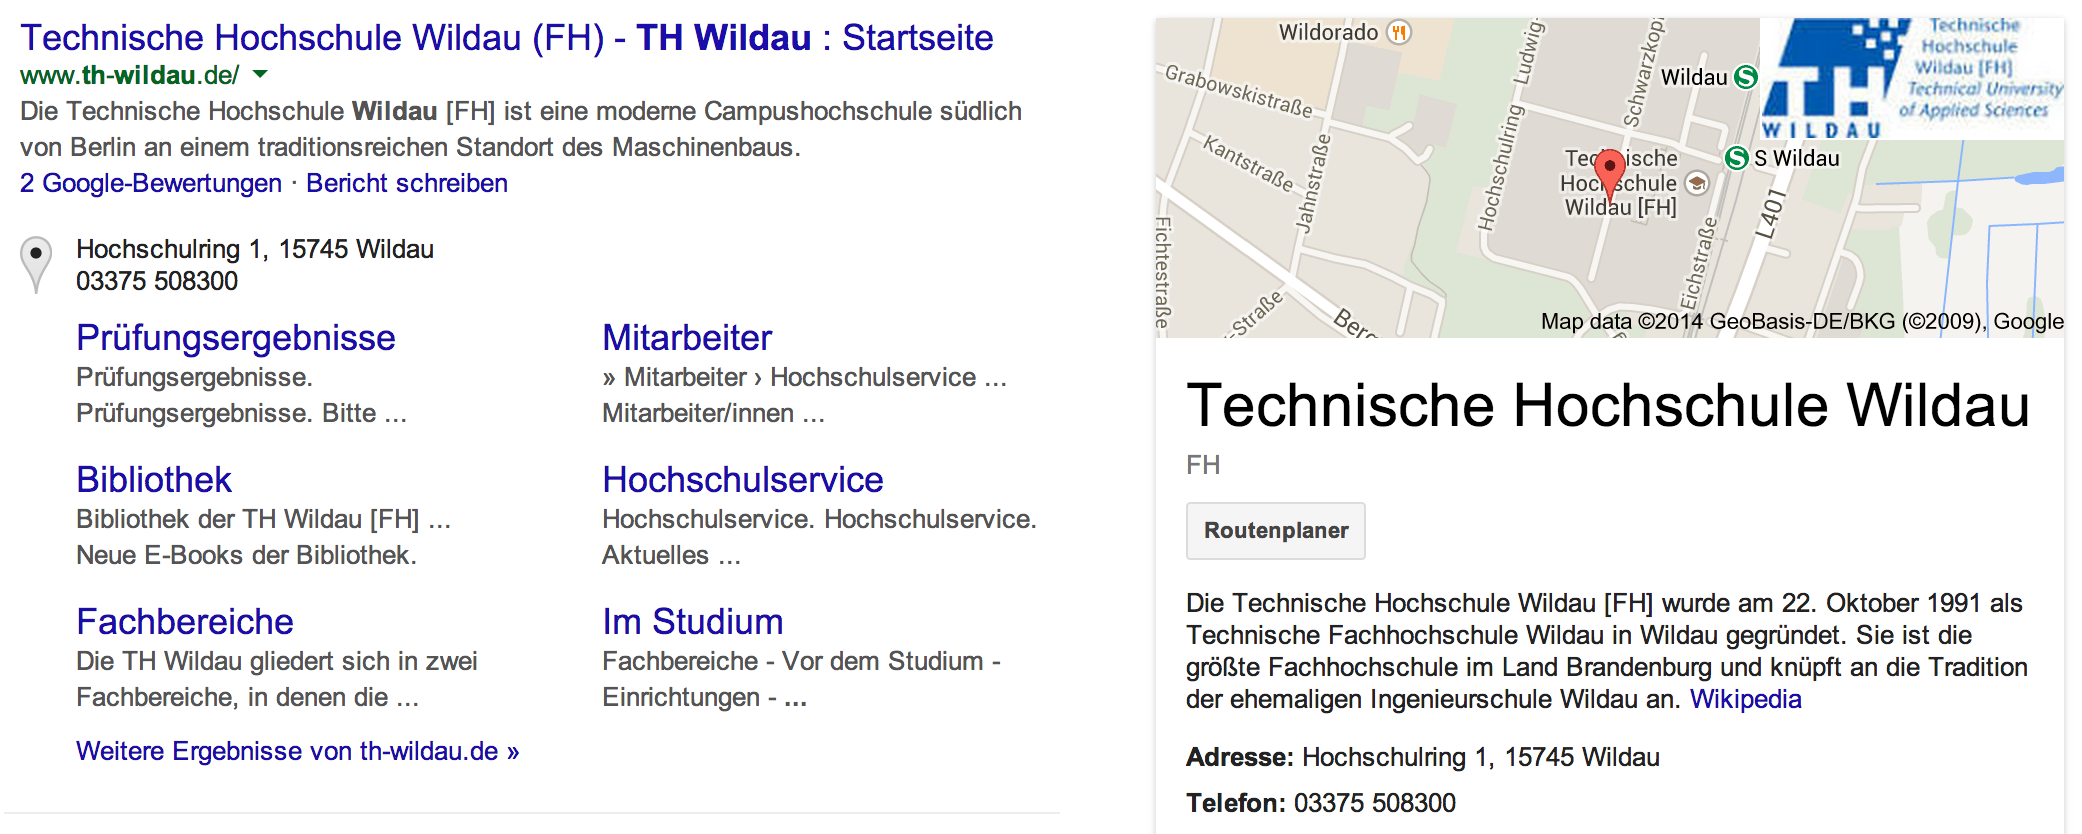
\includegraphics[scale=0.4]{google-q-th-wildau-2014-05-26}
	\captionbelow{Screenshot von Google-Suche nach TH-Wildau am 2014-05-26}
	\label{fig:googleThWildau}
\end{figure}

\subsection{Quellcode}\label{quellcode}

%TODO
